\chapter{Preface}

\par
\sputnik is code for calculating a composite material structure. It is composed by two main codes called \macro and
\micro each one design for perfomed coupled calculation with themselves.

\chapter{Homogenization theory}
This chapter is aimed to explain the state of the art on homogenization theory. The main concepts where taken from
\cite{suquet_1985}.

\section{Introduction}

\begin{figure}[h!]
\resizebox{2cm}{!}{
 \documentclass{standalone}

\begin{document}

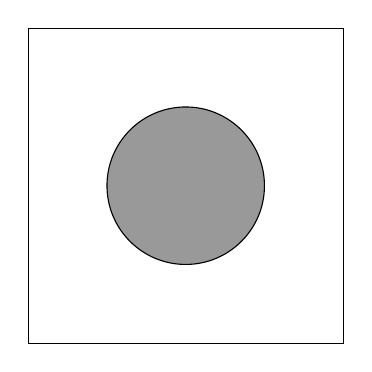
\begin{tikzpicture}

\draw (0,0) -- (4,0) -- (4,4) -- (0,4) -- cycle;
\filldraw[fill=black!40!white,draw=black] (2,2) circle (1cm);

\end{tikzpicture}

\end{document}


}
\end{figure}

\begin{figure}[h!]
\resizebox{5cm}{!}{
 \documentclass{standalone}

\begin{document}

\begin{tikzpicture}[>=latex,node distance=0pt]

\foreach \y [count=\n]in {0,4,8,12}{ 
  \foreach \x [count=\n]in {0,4,8,12}{ 
    \begin{scope}[yshift = \y cm,xshift = \x cm,start chain=going right]
      \draw (0,0) -- (4,0) -- (4,4) -- (0,4) -- cycle;
      \filldraw[fill=black!40!white,draw=black] (2,2) circle (1cm);
    \end{scope}
  }
}

\end{tikzpicture}

\end{document}


}
\end{figure}


\section{Localization and homogenization}

\begin{equation}
E_{ij} = \frac{1}{V}\int_{V}\epsilon_{ij}dy = \langle \epsilon_{ij} \rangle
\end{equation}

\begin{equation}
\Sigma_{ij} = \frac{1}{V}\int_{V}\sigma_{ij}dy = \langle \sigma_{ij} \rangle
\end{equation}

\subsection{Localization}


\subsection{Homogenization}



